% Source: Code/RADAR_web/docs/figures/fig_init_sequence.tex
\documentclass[border=5pt]{standalone}
\usepackage{tikz}
\usetikzlibrary{arrows.meta,positioning}
\usepackage{xcolor}

\definecolor{garnet}{HTML}{73000A}
\definecolor{black90}{HTML}{363636}
\definecolor{black70}{HTML}{5C5C5C}
\definecolor{black10}{HTML}{ECECEC}

\begin{document}
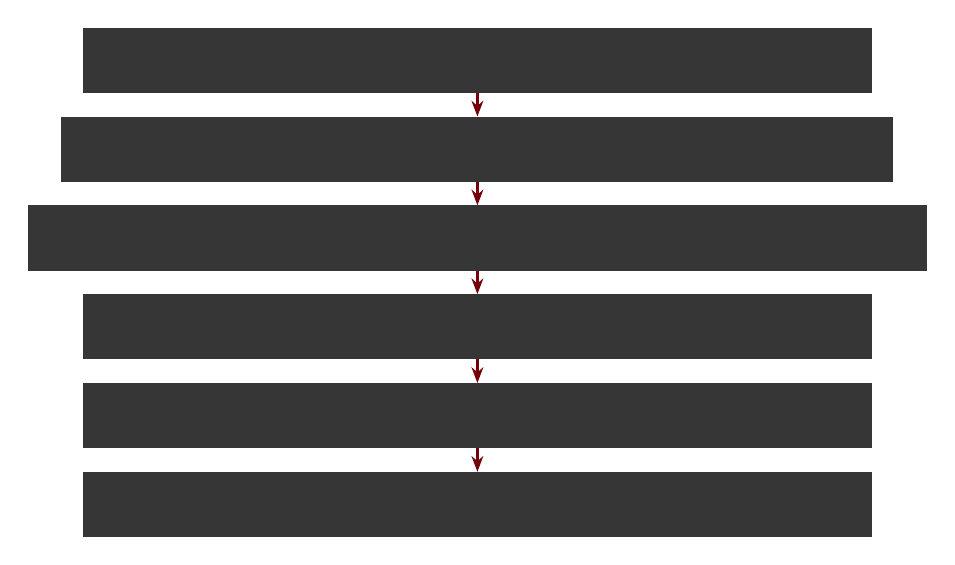
\begin{tikzpicture}[
    phase/.style={draw, thick, minimum width=10cm, minimum height=0.8cm, align=center, fill=black10, color=black90},
    arrow/.style={-{Stealth[length=2mm]}, thick, color=garnet},
    note/.style={font=\small\itshape, color=black70},
]

\node[phase] (p1) at (0,0) {\textbf{Phase 1:} Radar broadcasts beacon on UDP 10010};
\node[phase, below=0.3cm of p1] (p2) {\textbf{Phase 2:} TCP 10010 authentication (56-byte copyright exchange)};
\node[phase, below=0.3cm of p2] (p3) {\textbf{Phase 3:} TCP 10100 control channel open $\to$ \texttt{\$N00,CLIENTCONNECTION}};
\node[phase, below=0.3cm of p3] (p4) {\textbf{Phase 4:} Firmware query (\texttt{\$R96}) $\to$ version strings};
\node[phase, below=0.3cm of p4] (p5) {\textbf{Phase 5:} Bulk register reads (184 \texttt{\$R} commands)};
\node[phase, below=0.3cm of p5] (p6) {\textbf{Phase 6:} Ready for TX ON and echo data};

\foreach \i/\j in {p1/p2, p2/p3, p3/p4, p4/p5, p5/p6} {
    \draw[arrow] (\i.south) -- (\j.north);
}

\end{tikzpicture}
\end{document}
